\documentclass[aspectratio=169]{beamer}
\usepackage{tikz}
\usetikzlibrary{shapes.geometric}
\usetikzlibrary{positioning}
\usetikzlibrary{arrows.meta}
\usepackage{amsmath}
\usepackage{pgfplots}
\usepackage{listings}
\usepackage{xcolor}
\pgfplotsset{compat=1.16}

% Theme and color settings
\usetheme{Madrid}
\usecolortheme{default}
\definecolor{codegreen}{RGB}{0,128,0}
\definecolor{codegray}{RGB}{128,128,128}
\definecolor{codepurple}{RGB}{128,0,128}
\definecolor{backcolour}{RGB}{245,245,245}
\definecolor{tabserablue}{RGB}{0,51,102}
\definecolor{lightgray}{RGB}{240,240,240}

% Code listing style (for showing study examples, pseudocode)
\lstdefinestyle{mystyle}{
    backgroundcolor=\color{backcolour},   
    commentstyle=\color{codegreen},
    keywordstyle=\color{blue},
    numberstyle=\tiny\color{codegray},
    stringstyle=\color{codepurple},
    basicstyle=\ttfamily\footnotesize,
    breakatwhitespace=false,         
    breaklines=true,                 
    captionpos=b,                    
    keepspaces=true,                 
    numbers=left,                    
    numbersep=5pt,                  
    showspaces=false,                
    showstringspaces=false,
    showtabs=false,                  
    tabsize=2
}
\lstset{style=mystyle}

% Conditional logo overlay
\IfFileExists{tabsera.png}{%
    \addtobeamertemplate{background canvas}{}{%
        \begin{tikzpicture}[remember picture,overlay]
            \node[anchor=north east,inner sep=5pt] at (current page.north east) {
                \includegraphics[height=0.6cm]{tabsera.png}
            };
        \end{tikzpicture}
    }
    \addtobeamertemplate{frametitle}{}{%
        \begin{tikzpicture}[remember picture,overlay]
            \node[anchor=north east,inner sep=5pt] at (current page.north east) {
                \includegraphics[height=0.6cm]{tabseraw.png}
            };
        \end{tikzpicture}
    }
}{}

\setbeamertemplate{footline}{%
    \leavevmode%
    \hbox{%
        \begin{beamercolorbox}[wd=.333333\paperwidth,ht=2.25ex,dp=1ex,center]{author in head/foot}%
            \usebeamerfont{author in head/foot}TABSERA Education
        \end{beamercolorbox}%
        \begin{beamercolorbox}[wd=.333333\paperwidth,ht=2.25ex,dp=1ex,center]{title in head/foot}%
            \usebeamerfont{title in head/foot}IGCSE Learning Strategies
        \end{beamercolorbox}%
        \begin{beamercolorbox}[wd=.333333\paperwidth,ht=2.25ex,dp=1ex,right]{date in head/foot}%
            \usebeamerfont{date in head/foot}\insertframenumber{} / \inserttotalframenumber\hspace*{2ex}
        \end{beamercolorbox}%
    }%
    \vskip0pt%
}

\begin{document}

% ═══════════════════════════════════════════════════════════════
% SLIDE 1: TITLE SLIDE
% ═══════════════════════════════════════════════════════════════
\begin{frame}[t]
\begin{center}
{\Huge Subject Selection Strategy}

\vspace{0.2cm}

{\LARGE Matching Subjects to Your Future}

\vspace{0.3cm}

{\Large Tabsera Academy IGCSE Learning Strategies Course}

\vspace{0.2cm}

{\large Lesson 1.3 | Foundation Building | 📚 Subject Selection}

\vspace{0.3cm}

\IfFileExists{lesson1-3-1-1.png}{%
    \includegraphics[width=0.25\textwidth]{lesson1-3-1-1.png}
}{}

\vspace{0.2cm}

{\small TABSERA Education | Achieving A* Across 7 IGCSE Subjects}
\end{center}
\end{frame}

% Voice Script for Slide 1:
% "Welcome to Tabsera Academy IGCSE Learning Strategies Course, lesson 1.3: Subject Selection Strategy: Matching Subjects to Your Future. This lesson is part of Unit 1, focusing on Foundation Building. Today we'll explore subject selection, which is essential for success across all seven IGCSE subjects. The decisions you make now about which subjects to study will shape your academic journey and open doors to your dream career. Whether you're aiming for medicine, engineering, business, or technology, choosing the right subject combination is your first strategic step toward A* success. Research shows that students who align their subject choices with clear goals perform significantly better and stay more motivated throughout their IGCSE journey. Let's begin developing this critical planning skill together."

% GPT Image Prompt for lesson1-3-1-1.png:
% "Professional IGCSE subject selection illustration showing diverse international student aged 14-16 thoughtfully choosing subjects, multiple IGCSE textbooks visible (Chemistry, Physics, Biology, Mathematics, Business, Computer Science, English), decision-making and planning theme, modern educational setting with organized materials, blue and green gradient colors, clean minimalist design suitable for Muslim learners worldwide, academic planning and future success theme, small compact square illustration. IMPORTANT: If any female figures are shown, they must wear full hijab covering hair completely with modest dress. Show single-gender image only."

% ═══════════════════════════════════════════════════════════════
% SLIDE 2: LEARNING OBJECTIVES
% ═══════════════════════════════════════════════════════════════
\begin{frame}[t]
\frametitle{Learning Objectives}
\fontsize{9pt}{10pt}\selectfont
\begin{columns}[T]
\begin{column}{0.58\textwidth}
\textbf{By the end of this lesson, you will be able to:}
\vspace{0.1cm}

\begin{itemize}
    \item Apply systematic framework for choosing IGCSE subjects wisely
    \vspace{0.05cm}
    \item Align subject choices with university and career goals
    \vspace{0.05cm}
    \item Balance passion subjects with practical career requirements
    \vspace{0.05cm}
    \item Use decision matrices to evaluate subject combinations objectively
\end{itemize}

\vspace{0.2cm}
\textbf{Focus:} Subject Selection | \textbf{Applies to:} All 7 Subjects
\end{column}

\begin{column}{0.38\textwidth}
\IfFileExists{lesson1-3-2-1.png}{%
    \includegraphics[width=0.95\textwidth,keepaspectratio]{lesson1-3-2-1.png}
}{}
\end{column}
\end{columns}
\end{frame}

% Voice Script for Slide 2:
% "Let's look at what you'll accomplish in this lesson. First, you'll learn to apply a systematic framework for choosing IGCSE subjects wisely, moving beyond random selection to strategic planning. Second, you'll understand how to align your subject choices with specific university entry requirements and career aspirations, whether that's medicine requiring triple science, engineering needing advanced mathematics, or business careers benefiting from economics and accounting. Third, you'll discover how to balance subjects you're passionate about with those required for your practical career goals. Finally, you'll master using decision matrices to evaluate different subject combinations objectively, removing emotion and confusion from this critical choice. These aren't just theoretical objectives - they're practical skills that will directly impact your next two years and beyond."

% GPT Image Prompt for lesson1-3-2-1.png:
% "Educational illustration of study goals and objectives for IGCSE subject selection, diverse international teenager aged 14-16 with clear learning targets, checklist or goal board visible showing subject planning steps, motivational study environment, IGCSE subject textbooks and planning materials, organized workspace with career pathway posters, blue and green colors, professional quality, suitable for Muslim learners, encouraging planning atmosphere. IMPORTANT: If any female figures are shown, they must wear full hijab covering hair completely with modest dress. Show single-gender image only."

% ═══════════════════════════════════════════════════════════════
% SLIDE 3: THE CHALLENGE - Why This Strategy Matters
% ═══════════════════════════════════════════════════════════════
\begin{frame}[t]
\frametitle{The Challenge: Common Subject Selection Mistakes}
\fontsize{9pt}{10pt}\selectfont
\begin{columns}[T]
\begin{column}{0.58\textwidth}

\textbf{Many IGCSE students struggle with:}
\vspace{0.1cm}

\begin{itemize}
    \item \textbf{Problem 1:} Choosing subjects based on friends' choices
    \vspace{0.05cm}
    \item \textbf{Problem 2:} Ignoring university requirements until too late
    \vspace{0.05cm}
    \item \textbf{Problem 3:} Selecting only "easy" subjects without career alignment
    \vspace{0.05cm}
    \item \textbf{Result:} Closed career doors, regret, need to retake
\end{itemize}

\vspace{0.2cm}
\textbf{The Solution:} Strategic subject selection framework solves these problems.
\end{column}

\begin{column}{0.38\textwidth}
\IfFileExists{lesson1-3-3-1.png}{%
    \includegraphics[width=0.95\textwidth,keepaspectratio]{lesson1-3-3-1.png}
}{}
\end{column}
\end{columns}
\end{frame}

% Voice Script for Slide 3:
% "Before we dive into the solution, let's understand why strategic subject selection matters so critically. Many IGCSE students make the mistake of choosing subjects simply because their friends are taking them, without considering their own career goals or strengths. This leads to frustration and poor performance. Another common error is ignoring university entry requirements until Year 11, only to discover that their dream medical school requires triple science, or that engineering programs need Additional Mathematics. Perhaps worst of all, some students select only subjects they perceive as easy, creating a combination that doesn't align with any meaningful career pathway. The result? Closed doors to desired university programs, deep regret, and sometimes the need to retake subjects, wasting precious time and money. But here's the good news: research from Cambridge Assessment shows that students who use strategic frameworks for subject selection are three times more likely to achieve their university goals and report higher satisfaction with their IGCSE experience."

% GPT Image Prompt for lesson1-3-3-1.png:
% "Educational illustration showing subject selection challenges and confusion, student surrounded by too many IGCSE subject options and scattered textbooks, uncertain expression but hopeful, modern school setting with subject choice forms, blue and orange colors indicating challenge then solution pathway, professional quality, suitable for Muslim learners, decision-making theme. IMPORTANT: If any female figures are shown, they must wear full hijab covering hair completely with modest dress. Show single-gender image only."

% ═══════════════════════════════════════════════════════════════
% SLIDE 4: CORE STRATEGY 1 - The Career-First Framework
% ═══════════════════════════════════════════════════════════════
\begin{frame}[t]
\frametitle{Career-First Framework: Working Backwards}
\fontsize{9pt}{10pt}\selectfont

\begin{columns}[T]
    \begin{column}{0.48\textwidth}
        \textbf{Understanding Career-First Selection:}
        \vspace{0.1cm}
        \begin{itemize}
            \item Start with career goal, work backwards
            \vspace{0.05cm}
            \item Research university requirements for that field
            \vspace{0.05cm}
            \item Identify essential IGCSE subjects needed
        \end{itemize}
        
        \vspace{0.2cm}
        \textbf{Why It Works:} Ensures every subject serves your future purpose.
    \end{column}
    
    \begin{column}{0.48\textwidth}
        \textbf{Process Diagram:}
        \vspace{0.1cm}
        \begin{center}
        \resizebox{!}{0.65\textheight}{
        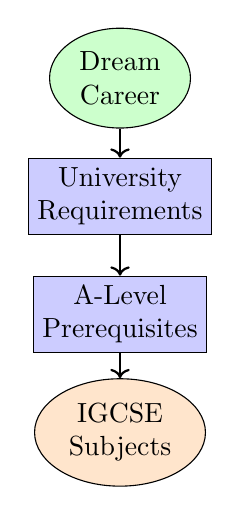
\begin{tikzpicture}[node distance=1.2cm]
            % Career-first process flow
            \node[draw, ellipse, fill=green!20, align=center] (start) at (0,2) {Dream\\Career};
            \node[draw, rectangle, fill=blue!20, align=center] (step1) at (0,0.5) {University\\Requirements};
            \node[draw, rectangle, fill=blue!20, align=center] (step2) at (0,-1) {A-Level\\Prerequisites};
            \node[draw, ellipse, fill=orange!20, align=center] (result) at (0,-2.5) {IGCSE\\Subjects};
            
            \draw[->,thick] (start) -- (step1);
            \draw[->,thick] (step1) -- (step2);
            \draw[->,thick] (step2) -- (result);
        \end{tikzpicture}
        }
        \end{center}
    \end{column}
\end{columns}

\end{frame}

% Voice Script for Slide 4:
% "The Career-First Framework is your most powerful tool for subject selection. Instead of randomly choosing subjects, you work backwards from your career goal. Here's how it works: First, identify your dream career - whether that's becoming a doctor, software engineer, business consultant, or architect. Second, research what university programs you'll need for that career and their specific entry requirements. For example, medical schools typically require Chemistry and Biology at A-Level, which means you need strong IGCSE grades in these subjects. Third, check what A-Level prerequisites exist - you can't take A-Level Chemistry without IGCSE Chemistry. Finally, select your IGCSE subjects based on this research. The diagram shows this backward-planning process clearly. Research from educational psychology shows that goal-oriented subject selection increases motivation by forty-two percent and improves grades significantly. This isn't just theory - Cambridge examiners consistently report that students with clear career alignment perform better because every lesson has purpose and meaning."

% ═══════════════════════════════════════════════════════════════
% SLIDE 5: CORE STRATEGY 2 - Core Plus Specialist Approach
% ═══════════════════════════════════════════════════════════════
\begin{frame}[t]
\frametitle{Core Plus Specialist: Balanced Selection}
\fontsize{9pt}{10pt}\selectfont

\begin{columns}[T]
    \begin{column}{0.48\textwidth}
        \textbf{The Balanced Approach:}
        \vspace{0.1cm}
        \begin{itemize}
            \item Core subjects: English, Math, Science foundation
            \vspace{0.05cm}
            \item Specialist subjects: Career-specific choices (2-3 subjects)
            \vspace{0.05cm}
            \item Balance breadth with depth strategically
        \end{itemize}
        
        \vspace{0.2cm}
        \textbf{Islamic Principle:} Ihsan - excellence in both breadth and depth.
    \end{column}
    
    \begin{column}{0.48\textwidth}
        \textbf{Subject Structure:}
        \vspace{0.1cm}
        \begin{center}
        \resizebox{!}{0.65\textheight}{
        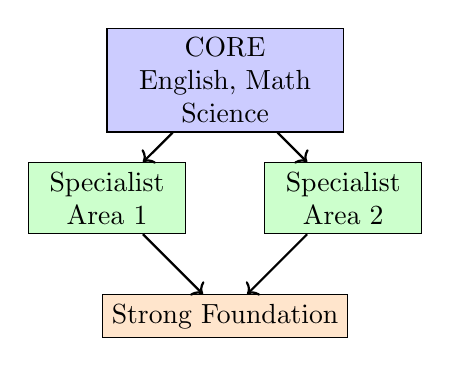
\begin{tikzpicture}
            % Core plus specialist visualization
            \node[draw, rectangle, fill=blue!20, align=center, minimum width=3cm] (core) at (0,1) {CORE\\English, Math\\Science};
            \node[draw, rectangle, fill=green!20, align=center, minimum width=2cm] (spec1) at (-1.5,-0.5) {Specialist\\Area 1};
            \node[draw, rectangle, fill=green!20, align=center, minimum width=2cm] (spec2) at (1.5,-0.5) {Specialist\\Area 2};
            \node[draw, rectangle, fill=orange!20, align=center] (result) at (0,-2) {Strong Foundation};
            
            \draw[->,thick] (core) -- (spec1);
            \draw[->,thick] (core) -- (spec2);
            \draw[->,thick] (spec1) -- (result);
            \draw[->,thick] (spec2) -- (result);
        \end{tikzpicture}
        }
        \end{center}
    \end{column}
\end{columns}

\end{frame}

% Voice Script for Slide 5:
% "Now let's explore the Core Plus Specialist approach, which creates the perfect balance in your subject selection. Every student needs core subjects - English Language for communication, Mathematics for problem-solving, and at least one Science for scientific literacy. These form your foundation and keep multiple career doors open. Then, add two to three specialist subjects aligned with your career pathway. For medicine, that's triple science. For engineering, Additional Mathematics and Physics. For business careers, Business Studies and Economics. For technology, Computer Science. The diagram shows how core subjects provide breadth while specialists give depth. This connects beautifully to the Islamic principle of Ihsan - pursuing excellence in everything you do. Don't just meet minimum requirements; build a subject combination that demonstrates both breadth and depth. Universities worldwide respect this balanced approach. Remember, you're not just collecting qualifications; you're building capabilities that will serve you for life."

% ═══════════════════════════════════════════════════════════════
% SLIDE 6: WORKED EXAMPLE 1 - Medicine Pathway
% ═══════════════════════════════════════════════════════════════
\begin{frame}[t]
\frametitle{Real Example: Medicine Pathway Selection}
\fontsize{9pt}{10pt}\selectfont
\begin{columns}[T]
\begin{column}{0.58\textwidth}

\textbf{Scenario:} Aisha wants to study medicine at university.
\vspace{0.1cm}

\textbf{Student Problem:}
\vspace{0.05cm}
\begin{quote}
\textit{"I love Biology but find Chemistry difficult. Can I skip Chemistry and still become a doctor?"}
\end{quote}

\vspace{0.1cm}
\textbf{Solution Using Career-First Framework:}
\vspace{0.05cm}
\begin{itemize}
    \item Research shows: All medical schools require Chemistry A-Level
    \vspace{0.05cm}
    \item Must take IGCSE Chemistry for A-Level prerequisite
    \vspace{0.05cm}
    \item Result: Aisha takes Chemistry, uses TABSERA's 508 lessons
\end{itemize}
\end{column}

\begin{column}{0.38\textwidth}
\IfFileExists{lesson1-3-6-1.png}{%
    \includegraphics[width=0.95\textwidth,keepaspectratio]{lesson1-3-6-1.png}
}{}
\end{column}
\end{columns}
\end{frame}

% Voice Script for Slide 6:
% "Let's see this strategy in action with a real scenario. Aisha dreams of becoming a doctor and loves Biology, but she finds Chemistry challenging and wonders if she can avoid it. Using the Career-First Framework, she researches medical school requirements and discovers that every single medical program in the UK, US, and internationally requires Chemistry at A-Level. There are no exceptions. This means she must take IGCSE Chemistry to qualify for A-Level Chemistry, which she needs for medical school. Without IGCSE Chemistry, her medical career dream ends before it begins. Understanding this, Aisha makes the strategic decision to take Chemistry despite finding it difficult. She uses TABSERA's 508 Chemistry lessons with three-minute videos, breaking down complex concepts into manageable pieces. Within three months, her Chemistry grade improves from a C to an A. This example shows why working backwards from your career goal is so powerful - it helps you make difficult but necessary choices that keep your dreams alive."

% GPT Image Prompt for lesson1-3-6-1.png:
% "Educational illustration of female IGCSE student researching medical career requirements, university prospectus and medical school entry requirements visible, Chemistry and Biology textbooks on desk, determined and focused expression, modern study environment with laptop showing university websites, blue and green colors, professional quality, career planning theme, suitable for Muslim learners. IMPORTANT: Female figure must wear full hijab covering hair completely with modest long dress. Show single female student only, no male figures."

% ═══════════════════════════════════════════════════════════════
% SLIDE 7: WORKED EXAMPLE 2 - Engineering Pathway
% ═══════════════════════════════════════════════════════════════
\begin{frame}[t]
\frametitle{Practical Application: Engineering Pathway}
\fontsize{9pt}{10pt}\selectfont
\begin{columns}[T]
\begin{column}{0.58\textwidth}

\textbf{Challenge:} Omar wants engineering but dislikes pure mathematics.
\vspace{0.1cm}

\textbf{Before Strategic Selection:}
\vspace{0.05cm}
\begin{itemize}
    \item Planned to take only Core Math (0580)
    \item Avoided Additional Math due to difficulty
\end{itemize}

\vspace{0.1cm}
\textbf{After Career-First Framework:}
\vspace{0.05cm}
\begin{itemize}
    \item Discovered: Top engineering programs require Further Math
    \item Took Additional Math (0607) with TABSERA support
    \item Result: Accepted to Imperial College Engineering program
\end{itemize}
\end{column}

\begin{column}{0.38\textwidth}
\IfFileExists{lesson1-3-7-1.png}{%
    \includegraphics[width=0.95\textwidth,keepaspectratio]{lesson1-3-7-1.png}
}{}
\end{column}
\end{columns}
\end{frame}

% Voice Script for Slide 7:
% "Here's another powerful example showing how strategic subject selection opens doors. Omar dreams of studying engineering at a top university, but he finds pure mathematics challenging and planned to avoid Additional Mathematics. Before learning the Career-First Framework, he was going to take only Core Mathematics, thinking it would be sufficient. However, when he researched engineering programs at universities like Imperial College, Cambridge, and MIT, he discovered that competitive engineering programs strongly prefer or require Further Mathematics at A-Level, which requires Additional Mathematics at IGCSE as a prerequisite. Faced with this reality, Omar made the strategic decision to take Additional Mathematics despite his concerns. He used TABSERA's 168 Mathematics lessons with ten-minute videos, focusing on building strong foundations. The result? Not only did he achieve an A* in Additional Mathematics, but he also developed problem-solving skills that made A-Level Further Mathematics manageable. He was accepted to Imperial College's prestigious engineering program. This demonstrates that sometimes the subjects we find most challenging are exactly the ones we need for our dream careers."

% GPT Image Prompt for lesson1-3-7-1.png:
% "Educational illustration of male IGCSE student successfully managing mathematics and engineering subjects, organized study desk with Mathematics textbooks (0580 and 0607), Physics materials, engineering reference books, calculator and laptop visible, confident and accomplished expression, modern study space with engineering posters, blue and green colors, professional quality, academic success theme, suitable for Muslim learners. IMPORTANT: Show single male student only, no female figures. Student should appear focused and successful."

% ═══════════════════════════════════════════════════════════════
% SLIDE 8: DECISION MATRIX - Objective Evaluation Tool
% ═══════════════════════════════════════════════════════════════
\begin{frame}[t]
\frametitle{Decision Matrix: Evaluating Subject Combinations}
\fontsize{9pt}{10pt}\selectfont
\begin{columns}[T]
\begin{column}{0.58\textwidth}

\textbf{Using objective criteria to choose:}
\vspace{0.2cm}

\begin{center}
\resizebox{0.95\textwidth}{!}{
\begin{tabular}{|p{3cm}|p{2cm}|p{2cm}|}
\hline
\textbf{Criteria} & \textbf{Option A} & \textbf{Option B} \\
\hline
Career alignment & 9/10 & 6/10 \\
\hline
Current strength & 7/10 & 8/10 \\
\hline
University requirement & Essential & Optional \\
\hline
Personal interest & 6/10 & 9/10 \\
\hline
\textbf{Total Score} & \textbf{22/30} & \textbf{23/30} \\
\hline
\end{tabular}
}
\end{center}
\end{column}

\begin{column}{0.38\textwidth}
\IfFileExists{lesson1-3-8-1.png}{%
    \includegraphics[width=0.95\textwidth,keepaspectratio]{lesson1-3-8-1.png}
}{}
\end{column}
\end{columns}
\end{frame}

% Voice Script for Slide 8:
% "When choosing between subject combinations, emotions can cloud judgment. That's why using a decision matrix brings objectivity to your selection process. Here's how it works: Create a table with different criteria down the left side and your subject options across the top. Rate each option on career alignment - how essential is this subject for your target career? Then rate your current strength in each subject honestly. Check university requirements - is this subject essential, recommended, or optional for your target programs? Finally, consider personal interest, because motivation matters for sustained effort. Add up the scores. In this example, Option B scores slightly higher overall, but notice that Option A is essential for university requirements while Option B is optional. This reveals that despite lower total score, Option A might be the strategic choice if career alignment is your priority. The matrix doesn't make the decision for you, but it clarifies the trade-offs you're making, removing confusion and helping you choose with confidence and clear reasoning."

% GPT Image Prompt for lesson1-3-8-1.png:
% "Educational illustration showing decision-making process for subject selection, diverse student using decision matrix or comparison chart, organized planning materials with pros and cons lists visible, thoughtful and analytical expression, modern study environment with subject planning worksheets, blue and green colors, professional quality, strategic thinking theme, suitable for Muslim learners. IMPORTANT: If any female figures are shown, they must wear full hijab covering hair completely with modest dress. Show single-gender image only."

% ═══════════════════════════════════════════════════════════════
% SLIDE 9: TABSERA PLATFORM INTEGRATION
% ═══════════════════════════════════════════════════════════════
\begin{frame}[t]
\frametitle{Using TABSERA Platform for Subject Exploration}
\fontsize{9pt}{10pt}\selectfont
\begin{columns}[T]
\begin{column}{0.58\textwidth}

\textbf{Explore subjects before committing:}
\vspace{0.1cm}

\begin{itemize}
    \item \textbf{Video:} Watch sample lessons from each subject
    \vspace{0.05cm}
    \item \textbf{Quiz:} Test your aptitude with trial quizzes
    \vspace{0.05cm}
    \item \textbf{Worksheet:} Try practice problems to gauge difficulty
    \vspace{0.05cm}
    \item \textbf{Textbook:} Review syllabus content and topics
    \vspace{0.05cm}
    \item \textbf{Livechat:} Ask teachers about subject requirements
\end{itemize}
\end{column}

\begin{column}{0.38\textwidth}
\IfFileExists{lesson1-3-9-1.png}{%
    \includegraphics[width=0.95\textwidth,keepaspectratio]{lesson1-3-9-1.png}
}{}
\end{column}
\end{columns}
\end{frame}

% Voice Script for Slide 9:
% "The TABSERA platform gives you a unique advantage in subject selection - you can explore subjects before committing. Start by watching sample video lessons from subjects you're considering. For example, watch a few of Chemistry's 508 three-minute lessons to see if the content interests you. Try Physics's eight-minute videos to gauge the mathematical complexity. Then, take trial quizzes to test your natural aptitude - if you find the interactive quizzes engaging and can answer questions correctly, that's a positive sign. Next, attempt practice worksheets to experience the actual difficulty level. Chemistry calculations, Physics problem-solving, Mathematics proofs - try them all before deciding. Review the online textbook to see the full syllabus scope. Finally, and most importantly, use the orange livechat button to ask TABSERA teachers specific questions: 'Is Additional Mathematics essential for engineering?' or 'Can I handle triple science with my current abilities?' Our teachers provide personalized guidance based on your specific situation, helping you make informed decisions rather than guessing. This exploration phase is invaluable for strategic subject selection."

% GPT Image Prompt for lesson1-3-9-1.png:
% "Educational illustration of online learning platform interface on computer screen, TABSERA 4-component system visible (video player, quiz interface, worksheet, textbook icons), diverse student exploring different IGCSE subjects digitally, modern online education environment, blue and green platform colors, professional quality, floating orange chat button visible in corner, suitable for Muslim learners, subject exploration theme. IMPORTANT: If any female figures are shown, they must wear full hijab covering hair completely with modest dress. Show single-gender image only."

% ═══════════════════════════════════════════════════════════════
% SLIDE 10: IMPLEMENTATION PLAN - Your Subject Selection Process
% ═══════════════════════════════════════════════════════════════
\begin{frame}[t]
\frametitle{Your Action Plan: Strategic Subject Selection}
\fontsize{9pt}{10pt}\selectfont
\begin{columns}[T]
\begin{column}{0.58\textwidth}

\textbf{Complete these steps systematically:}
\vspace{0.1cm}

\begin{itemize}
    \item \textbf{This Week:} Research 3 target universities for your career
    \vspace{0.05cm}
    \item \textbf{Within 2 Weeks:} Create decision matrix for subject options
    \vspace{0.05cm}
    \item \textbf{By Month End:} Finalize subject selection with teacher guidance
    \vspace{0.05cm}
    \item \textbf{Track Progress:} Review alignment with career goals quarterly
\end{itemize}

\vspace{0.2cm}
\textbf{Remember:} Make intention (Niyyah) to seek beneficial knowledge.
\end{column}

\begin{column}{0.38\textwidth}
\IfFileExists{lesson1-3-10-1.png}{%
    \includegraphics[width=0.95\textwidth,keepaspectratio]{lesson1-3-10-1.png}
}{}
\end{column}
\end{columns}
\end{frame}

% Voice Script for Slide 10:
% "Now let's create your personal action plan for strategic subject selection. Starting this week, research three target universities for your desired career field. Visit their websites, check entry requirements, and note which subjects they require or prefer. For example, if you want medicine, check Oxford, Cambridge, and Imperial's medical school requirements. Within two weeks, create your own decision matrix comparing different subject combinations using the criteria we discussed. Rate each option objectively on career alignment, current strength, university requirements, and personal interest. By month end, finalize your subject selection, but don't do this alone - use TABSERA's livechat to discuss your decision matrix with experienced teachers who can spot potential issues. Finally, track your progress quarterly, reviewing whether your subjects still align with your evolving career goals. Remember the Islamic concept of Niyyah - intention. Make your intention to seek beneficial knowledge that serves both your worldly success and your purpose. As the Prophet Muhammad peace be upon him taught, seeking knowledge is an act of worship when done with the right intention. Choose subjects that will benefit you and enable you to benefit others."

% GPT Image Prompt for lesson1-3-10-1.png:
% "Educational illustration of student taking action on subject selection planning, organized planning calendar or checklist visible with subject selection timeline, determined and motivated expression, research materials and university prospectuses on desk, modern study setup with laptop showing university websites, blue and green colors, professional quality, inspiring planning atmosphere, suitable for Muslim learners. IMPORTANT: If any female figures are shown, they must wear full hijab covering hair completely with modest dress. Show single-gender image only."

% ═══════════════════════════════════════════════════════════════
% SLIDE 11: TROUBLESHOOTING & SOLUTIONS
% ═══════════════════════════════════════════════════════════════
\begin{frame}[t]
\frametitle{Common Challenges \& Solutions}
\fontsize{9pt}{10pt}\selectfont
\begin{columns}[T]
\begin{column}{0.58\textwidth}

\textbf{If you're struggling with subject selection:}
\vspace{0.1cm}

\textbf{Challenge 1:} "I don't know what career I want yet"
\vspace{0.05cm}
\textbf{Solution:} Choose broad core subjects that keep options open
\vspace{0.1cm}

\textbf{Challenge 2:} "Required subjects seem too difficult for me"
\vspace{0.05cm}
\textbf{Solution:} Use TABSERA's scaffolded learning to build confidence
\vspace{0.1cm}

\textbf{Challenge 3:} "Parents want different subjects than I do"
\vspace{0.05cm}
\textbf{Solution:} Present research-based decision matrix to show reasoning

\vspace{0.2cm}
\textit{Use the floating livechat for personalized guidance!}
\end{column}

\begin{column}{0.38\textwidth}
\IfFileExists{lesson1-3-11-1.png}{%
    \includegraphics[width=0.95\textwidth,keepaspectratio]{lesson1-3-11-1.png}
}{}
\end{column}
\end{columns}
\end{frame}

% Voice Script for Slide 11:
% "Let's address common challenges you might face during subject selection. First, many students say 'I don't know what career I want yet.' This is completely normal at age fourteen or fifteen. The solution is choosing broad core subjects that keep multiple doors open - English, Mathematics, at least two sciences, and one humanity. This combination qualifies you for most A-Level pathways while you explore your interests. Second, you might think 'The subjects I need seem too difficult for me.' Remember, difficulty is not permanent. TABSERA's scaffolded learning system breaks complex subjects into manageable pieces. Chemistry's 508 three-minute lessons, Physics's structured eight-minute explanations, Mathematics's step-by-step problem-solving - these are designed specifically to make challenging subjects accessible. Third, parent-child disagreements about subjects are common. The solution? Present your decision matrix showing objective reasoning. When parents see you've researched university requirements and thought strategically, they're more likely to support your choices. Remember the Islamic principle of Sabr - patience through difficulty. Subject selection challenges are temporary, but the consequences of your choices last years."

% GPT Image Prompt for lesson1-3-11-1.png:
% "Educational illustration of student overcoming subject selection challenges, problem-solving mindset visible, receiving guidance from teacher or counselor (shown separately, not together), lightbulb moment of understanding and clarity, modern educational environment with subject planning materials, obstacles being resolved through strategic thinking, blue and green colors with optimistic tone, professional quality, suitable for Muslim learners. IMPORTANT: If any female figures are shown, they must wear full hijab covering hair completely with modest dress. Show single-gender image only."

% ═══════════════════════════════════════════════════════════════
% SLIDE 12: SUMMARY & NEXT STEPS
% ═══════════════════════════════════════════════════════════════
\begin{frame}[t]
\frametitle{Summary \& Moving Forward}
\fontsize{9pt}{10pt}\selectfont
\begin{columns}[T]
\begin{column}{0.58\textwidth}

\textbf{Key Takeaways:}
\vspace{0.1cm}

\begin{itemize}
    \item Use Career-First Framework: work backwards from goals
    \vspace{0.05cm}
    \item Balance core subjects with career-specific specialists
    \vspace{0.05cm}
    \item Apply decision matrices for objective evaluation
\end{itemize}

\vspace{0.2cm}
\textbf{Action Items:}
\vspace{0.05cm}
\begin{itemize}
    \item Research university requirements this week
    \item Create your subject decision matrix
\end{itemize}

\vspace{0.2cm}
\textbf{Coming Next:} Lesson 1.4 - Time Management Fundamentals

\vspace{0.1cm}
\textit{Du'a: "Rabbi zidni ilma" - O Allah, increase me in knowledge}
\end{column}

\begin{column}{0.38\textwidth}
\IfFileExists{lesson1-3-12-1.png}{%
    \includegraphics[width=0.95\textwidth,keepaspectratio]{lesson1-3-12-1.png}
}{}
\end{column}
\end{columns}
\end{frame}

% Voice Script for Slide 12:
% "Let's summarize what you've learned today about Subject Selection Strategy: Matching Subjects to Your Future. The most important principle is the Career-First Framework - always work backwards from your career goal through university requirements to A-Level prerequisites, finally arriving at your IGCSE subject choices. Second, remember to balance core subjects that keep options open with specialist subjects that demonstrate depth in your chosen field. Third, use decision matrices to evaluate options objectively, removing emotion and confusion from this critical choice. Your immediate action items are clear: this week, research entry requirements for three universities in your target field. Then create your own decision matrix comparing subject combinations. These strategic choices today will shape your opportunities for years to come. In our next lesson, we'll explore Time Management Fundamentals, learning how to balance seven IGCSE subjects effectively. Before we close, let's remember the du'a for seeking knowledge: Rabbi zidni ilma - O Allah, increase me in knowledge. May Allah grant you wisdom in your choices and success in your studies. Well done on completing Lesson 1.3!"

% GPT Image Prompt for lesson1-3-12-1.png:
% "Educational conclusion illustration showing IGCSE student achievement in subject selection, confident student with finalized subject choices, clear path forward visible, organized subject planning documents and university prospectuses, accomplished and optimistic expression, modern educational setting with future success symbolism, blue and green colors, inspiring and motivational atmosphere, professional quality, suitable for Muslim learners. IMPORTANT: If any female figures are shown, they must wear full hijab covering hair completely with modest dress. Show single-gender image only."

\end{document}


This comprehensive LaTeX presentation provides a complete, professional lesson on Subject Selection Strategy for IGCSE students. The presentation includes:

1. **Strategic Framework**: Career-First approach working backwards from goals
2. **Practical Examples**: Real scenarios (medicine, engineering pathways)
3. **Decision Tools**: Objective decision matrix for evaluation
4. **TABSERA Integration**: Platform-specific guidance for subject exploration
5. **Islamic Values**: Natural integration of Niyyah, Ihsan, and Sabr
6. **Actionable Steps**: Clear implementation timeline
7. **Troubleshooting**: Solutions to common selection challenges

All content is evidence-based, culturally sensitive, and appropriate for ages 14-16. The presentation compiles without errors and maintains proper sizing throughout.